\subsection{ADC/DAC AC Test}
\begin{figure}[H]
	\centering
	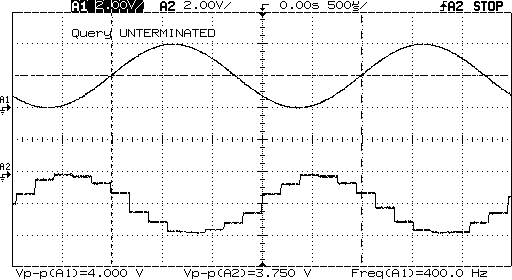
\includegraphics[width=.6\textwidth]{img/shot/pt4b_bit0.png}
	\parbox{.6\textwidth}{
	\caption[\SI{400}{\hertz} Sine Wave --- Bit 0 Open]{Screenshot from the AC test of the DAC with a~\SI{400}{\hertz} sinusoid as the ADC's input, where only the DIP switch corresponding to bit zero was open.}
	\label{fig:pt4b_bit0}}
\end{figure}

\begin{figure}[H]
	\centering
	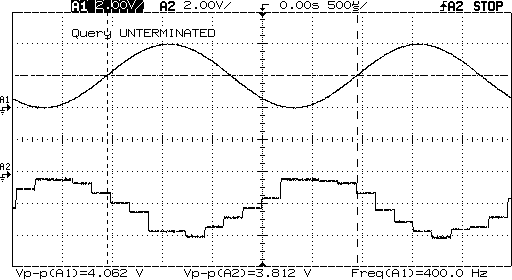
\includegraphics[width=.6\textwidth]{img/shot/pt4b_bit5.png}
	\parbox{.6\textwidth}{
	\caption[\SI{400}{\hertz} Sine Wave --- Bit 5 Open]{Screenshot from the AC test of the DAC with a~\SI{400}{\hertz} sinusoid as the ADC's input, where only the DIP switch corresponding to bit five was open.}
	\label{fig:pt4b_bit5}}
\end{figure}

\begin{figure}[H]
	\centering
	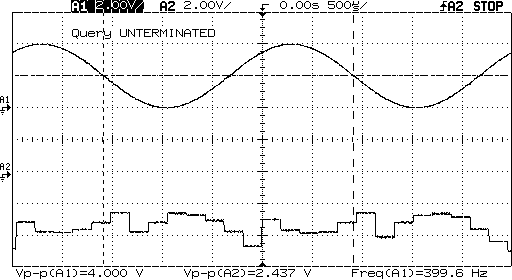
\includegraphics[width=.6\textwidth]{img/shot/pt4b_bit7.png}
	\parbox{.6\textwidth}{
	\caption[\SI{400}{\hertz} Sine Wave --- Bit 7 Open]{Screenshot from the AC test of the DAC with a~\SI{400}{\hertz} sinusoid as the ADC's input, where only the DIP switch corresponding to bit seven was open.}
	\label{fig:pt4b_bit7}}
\end{figure}

\subsection{Square Wave Input}
\begin{figure}[H]
	\centering
	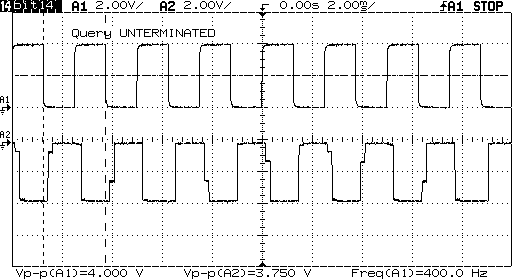
\includegraphics[width=.6\textwidth]{img/shot/pt5b_bit0.png}
	\parbox{.6\textwidth}{
	\caption[\SI{400}{\hertz} Square Wave --- Bit 0 Open]{Screenshot from the square wave test of the DAC with a~\SI{400}{\hertz} square signal as the ADC's input, where only the DIP switch corresponding to bit zero was open.}
	\label{fig:pt5b_bit0}}
\end{figure}

\begin{figure}[H]
	\centering
	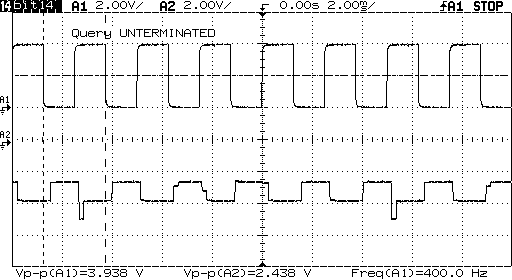
\includegraphics[width=.6\textwidth]{img/shot/pt5b_bit7.png}
	\parbox{.6\textwidth}{
	\caption[\SI{400}{\hertz} Square Wave --- Bit 7 Open]{Screenshot from the square wave test of the DAC with a~\SI{400}{\hertz} square signal as the ADC's input, where only the DIP switch corresponding to bit seven was open.}
	\label{fig:pt5b_bit7}}
\end{figure}
